\subsection{Higher research productivity}
\label{subsec:rewrite-rsi-half-decline}

I first ask how research, consumption, and capital accumulation respond
when RSI becomes available under an existing monopoly, and how this
adjustment differs across economies approaching the two long-run regimes.
I compare the four elasticities under relatively high research
productivity, $\chi=7.5$. Research productivity
affects the transition, but not the limiting growth rates characterized in
Section~\ref{sec:rewrite-regimes}. All four economies inherit the pre-RSI
balanced growth paths described in Section~\ref{subsec:rewrite-rsi-activation}.
Table~\ref{tab:rewrite-rsi-parameters} reports their common parameters and
elasticity-specific initial capital stocks. I examine quantities first,
then wages and prices, and finally income shares.

% The generated numerical digest in rsi_chi_7_5_results.tex is retained,
% but not input here: editorial prose is organized around the three figures.
% Source: numerical_rewrite/rsi_chi_7_5/{summary,figure_manifest}.json.
I use Figure~\ref{fig:rewrite-rsi-half-accumulation} to present the annual growth rates of output, AI production services, and capital per unit of effective labor: $Y/(AL)$, $X/(AL)$, and $K/(AL)$. Zero therefore means that the corresponding aggregate grows at the same rate as effective labor, $n+\gamma$. The upper row shows two pre-event years and the first ten years after RSI activation. The lower row follows the same variables from year 10 to year 500. Throughout the three figures, green dashed, black solid, orange dotted, and blue dash-dotted lines denote $\sigma=0.90,1,1.10,1.50$, respectively. The vertical line marks RSI activation, and black dotted horizontal lines mark the analytical
limits for $\sigma=1.50$. %Vertical scales differ across time windows.

\begin{figure}[H]
 \centering
 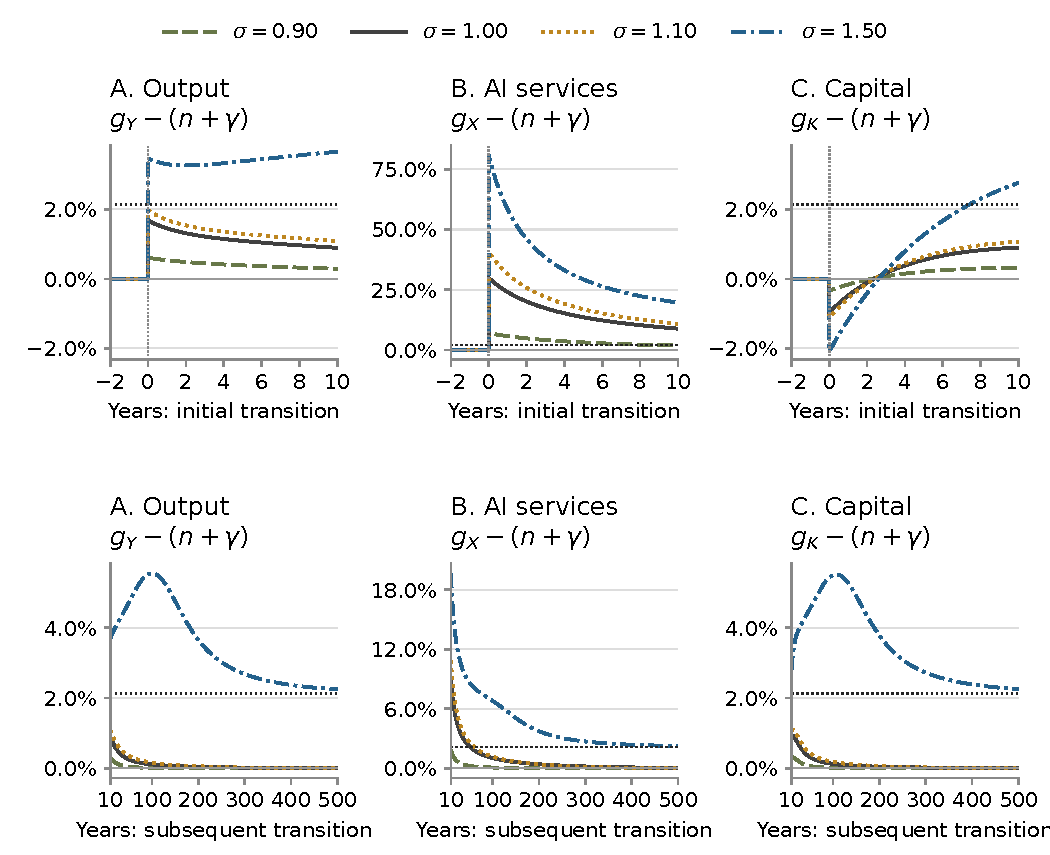
\includegraphics[width=\textwidth]{figures_rewrite/equilibrium_rsi_chi_7_5_accumulation_growth_windows.pdf}
 \caption{Higher research productivity ($\chi=7.5$): growth of output,
 AI production services, and capital per unit of effective labor. Rates
 are instantaneous annual rates. The upper row shows two pre-event years
 and years 0--10; the lower row shows years 10--500. Panels A and C share
 a scale within each row. The vertical line marks RSI activation.}
 \label{fig:rewrite-rsi-half-accumulation}
\end{figure}


The top row of Figure~\ref{fig:rewrite-rsi-half-accumulation} shows that AI services respond much more strongly than output. At $\sigma=1.50$, $X/(AL)$ initially grows at $80.8\%$ per year, whereas $Y/(AL)$ grows at $3.5\%$. Research begins to raise $B$, allowing more services to be obtained from compute through $X=BU$. Final production cannot expand at the same rate because it also requires capital and labor. Initial growth of $Y/(AL)$ is smaller at the other elasticities, reaching only $0.6\%$ at $\sigma=0.90$. The third panel shows the capital response: capital per unit of effective labor, $K/(AL)$, falls in every case. Households increase consumption at RSI activation while the developer starts spending on research. The resource constraint thus requires lower investment in physical capital. Capital accumulation
subsequently recovers as output expands and as the marginal product of capital increases.

The bottom row of Figure~\ref{fig:rewrite-rsi-half-accumulation} separates temporary growth gains from permanent ones. At $\sigma=0.90,1,1.10$, all three normalized growth rates decline
toward zero. This is the labor-bottleneck outcome in
Proposition~\ref{prop:rewrite-equilibrium-regimes}: output per worker eventually grows at $\gamma=1.0\%$. At $\sigma=1.50$, output and capital
growth instead rise further before declining toward their long-run values.
As explained in Section~\ref{subsec:rewrite-equilibrium-existence},
sufficient substitution and a sufficiently high efficiency bound allow
capital and inference compute to expand together without being limited
by effective-labor growth. Their limiting growth rates exceed effective-labor growth by $2.1$ percentage points; effective labor itself grows at $1.3\%$ per year.

I next examine wages and prices in Figure~\ref{fig:rewrite-rsi-half-prices}. The figure shows annual wage growth $g_w$, the annual net interest rate $r$, and the level of $p_X$ in final-good units on a logarithmic scale. The top panels present the short-run dynamics and the bottom panels present the long-run dynamics. Wage growth increases in all four economies, but the initial response is not ordered monotonically by substitutability: the immediate increase is larger at $\sigma=1$ than at $\sigma=1.50$. Wage growth in the highest-elasticity case soon surpasses the other cases. After the initial jump, wage growth declines in the labor-bottleneck cases but continues to rise in the AI-dominated case. Meanwhile, the interest rate starts at $5.0\%$ in every case and then rises as output initially outpaces capital. The higher return accompanies faster consumption-per-person growth, as required by the Euler condition in Equation~\eqref{eq:rewrite-euler}. A related mechanism underlies \citet{chowhalperinmazlish2026}, who link faster expected consumption growth to higher long-term real interest rates. Meanwhile, $p_X$ falls continuously as AI efficiency improves. %The pricing condition \eqref{eq:rewrite-eq-monopoly} links the price to the compute cost per service, $1/B$, and the markup. At unit elasticity the markup is constant, so the price falls in inverse proportion to $B$; its decline over the first 27 months is $39.6\%$, an outcome rather than a calibration target.

The bottom row of Figure~\ref{fig:rewrite-rsi-half-prices} shows the longer adjustment of wage growth, the interest rate, and the AI-service price. The three labor-bottleneck economies return toward wage growth of $1.0\%$ and an interest rate of $5.0\%$. At $\sigma=1.50$, both rates rise above their long-run values before declining. Equation~\eqref{eq:rewrite-substitutes-wage-growth} gives limiting wage growth of $2.4\%$, below output-per-worker growth of $3.1\%$ but above labor-augmenting technological progress of $1.0\%$. Meanwhile, the interest rate tends to $\mathcal R(\overline B)=7.1\%$, above its pre-RSI level. %At year 500, the corresponding wage growth and interest rate are still $2.5\%$ and $7.2\%$. The price approaches a positive level in every case, rather than falling forever at a constant proportional rate. In the AI-dominated limit, $s_X\to1$ and $e_X\to\alpha$, so the pricing condition gives $p_X\to1/[(1-\alpha)\overline B]\simeq0.00110$.

\begin{figure}[H]
 \centering
 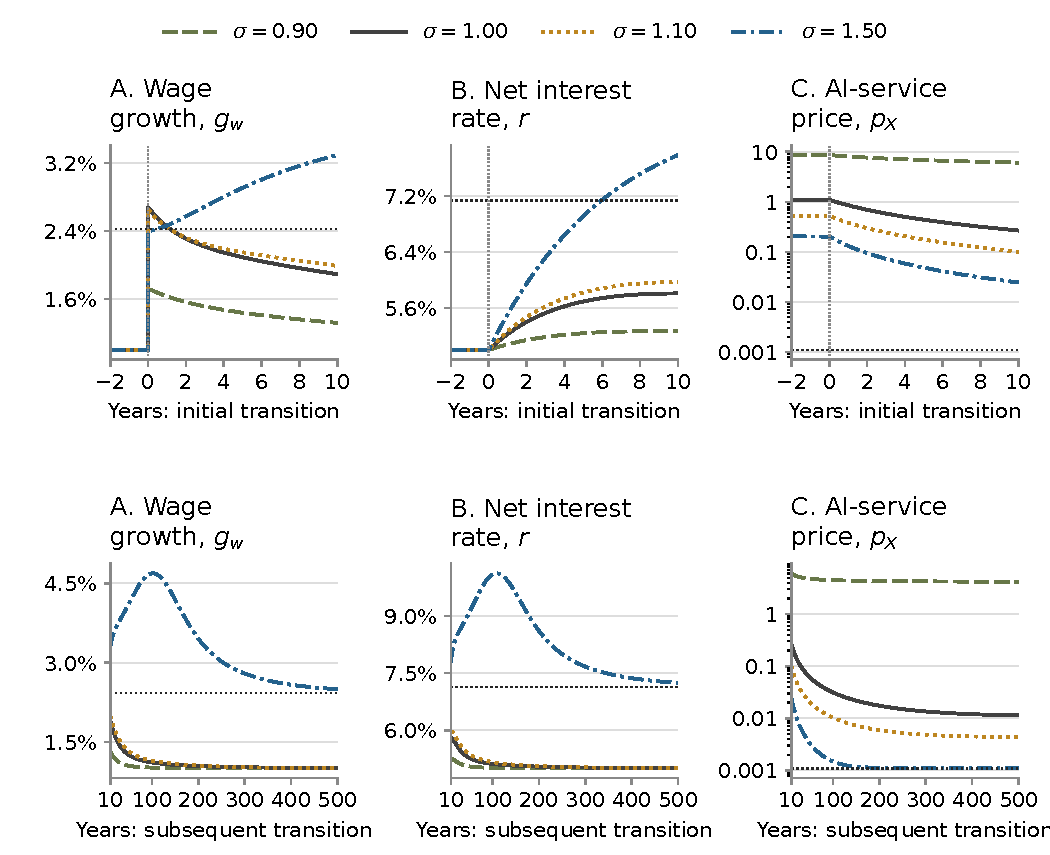
\includegraphics[width=\textwidth]{figures_rewrite/equilibrium_rsi_chi_7_5_growth_returns_windows.pdf}
 \caption{Higher research productivity ($\chi=7.5$): wage growth,
 the net interest rate, and the AI-service price. Rates are annual;
 the price is in final-good units on a logarithmic scale.
 The vertical line marks RSI activation.}
 \label{fig:rewrite-rsi-half-prices}
\end{figure}

Finally, I use Figure~\ref{fig:rewrite-rsi-half-distribution} to show labor income $wL/Y$, developer net profit $\Pi/Y$, inference expenditure $U/Y$, and research expenditure $M/Y$, all as a share of output. The top four panels show the short run and the bottom four panels show the long run. Line styles again identify the four elasticities. The omitted
gross capital income share remains $\alpha=33.0\%$.


\begin{figure}[H]
 \centering
 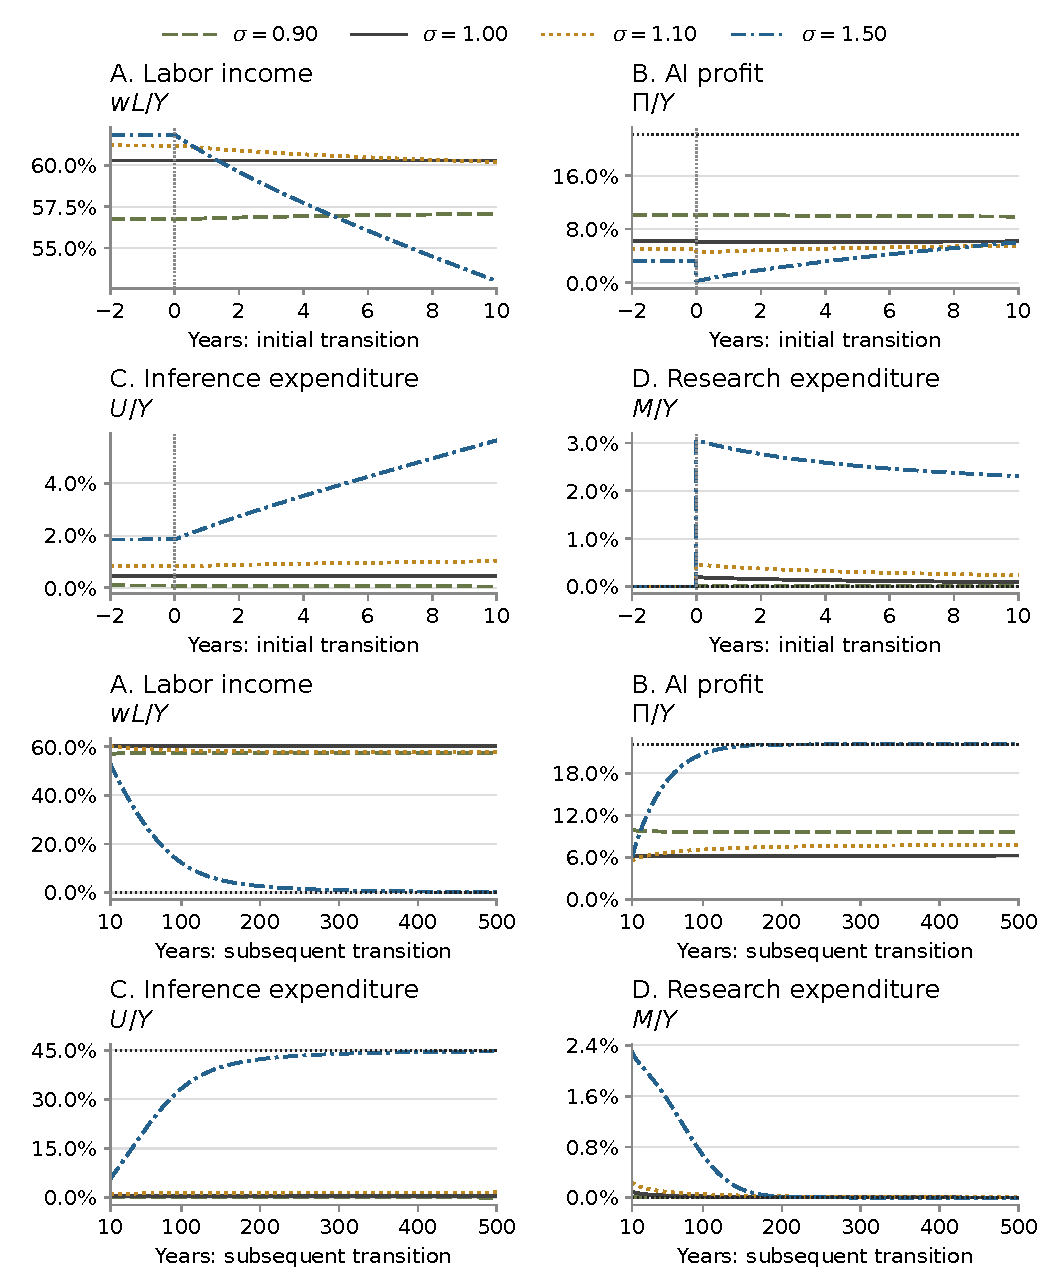
\includegraphics[width=\textwidth]{figures_rewrite/equilibrium_rsi_chi_7_5_ai_distribution_windows.pdf}
 \caption{Higher research productivity ($\chi=7.5$): labor income,
 AI net profit, inference expenditure, and research expenditure relative
 to output. The first two rows show the pre-event BGP and years 0--10;
 the last two show years 10--500. The omitted gross capital share
 remains $\alpha=0.33$. Short-run panels A and C use scales fitted to the
 initial trajectories and omit the long-run reference lines.}
 \label{fig:rewrite-rsi-half-distribution}
\end{figure}

In the short run, research spending as a share of output jumps in all four economies. The adjustment is strongest at $\sigma=1.50$: immediately after activation, research absorbs $59.4\%$ of AI revenue, compared with $35.9\%$ for inference compute. The developer's net profit therefore falls sharply. Profit subsequently recovers as research absorbs a smaller share of revenue and AI sales expand. Labor's income share also falls most strongly in this scenario, while changes are much smaller in the other three economies.

Over the longer horizon, the AI-dominated economy combines permanently faster wage growth with an even faster expansion of output per worker, so labor's income share tends to zero. Rising wages alongside a declining labor share also appear in \citet{autorkausik2026} and \citet{raymookherjee2022}. As labor's share falls, AI revenue rises relative to output. Inference compute eventually absorbs $67.0\%$ of AI revenue, while research expenditure vanishes relative to that revenue. These last proportions use AI revenue as the denominator, rather than output as in the figure.
